\documentclass{beamer}
\usetheme[block=fill]{metropolis}           % Use metropolis theme
\setbeamertemplate{section in toc}[sections numbered]
\setbeamertemplate{subsection in toc}[subsections numbered]

\usepackage[operators,sets]{cryptocode}
\usepackage{diagbox}
\usepackage{dashbox}

\newcommand{\cm}{\mathcal{C}} % polynomial commitment
\newcommand{\gs}{g_\mathsf{secp}} % the generator in secp256k1 group
\newcommand{\hs}{h_\mathsf{secp}} % another generator in secp256k1
\newcommand{\gb}{g_\mathsf{bls}} % the generator in BLS12-381 group
\newcommand{\hb}{h_\mathsf{bls}} % another generator in BLS12-381
\newcommand{\bls}{\texttt{bls12-381}}
\newcommand{\secp}{\texttt{secp256k1}}

\title{The Application of Zero-Knowledge Proofs: Proof of Solvency}
\date{\today}
\author{Youwei (Barry) Deng, Jeremy Clark}
\institute{Concordia University}

\AtBeginSection[]
{
  \begin{frame}{Table of Contents}
    \tableofcontents[currentsection]
  \end{frame}
}

\begin{document}
  \maketitle

  \section{Introduction}

  \subsection{What is ZKP}
  \begin{frame}{What is ZKP}
    \textbf{Goal:} Prove a statement is true without revealing additional information, only the fact itself.
    \visible<2->{
      \begin{itemize}
        \item Compared to classic proofs
        \begin{itemize}
          \item \textbf{Classic proofs} (pythagorean theorem, Euler's theorem, etc.): verifier passively reads the proof
          \item \textbf{ZKP}: two new ingredients, interaction and randomness
        \end{itemize}
      \end{itemize}
    }
    \vspace{-1em}
    \visible<3->{
      \begin{columns}
        \begin{column}{0.7\textwidth}
          \pseudocodeblock{
            \mathcal{P} \< \sendmessageright*{m_1} \< \mathcal{V} \\
            \< \sendmessageleft*{c_1\stackrel{\$}{\leftarrow}\{0,1\}^t} \\
            \< \sendmessageright*{m_2} \\
            \< \sendmessage*{<-}{top={c_2\stackrel{\$}{\leftarrow}\{0,1\}^t}, bottom={\dots}} \\
          }
        \end{column}

        \begin{column}{0.3\textwidth}
          interactive + probabilistic proof system
          \vspace*{4em}
        \end{column}
      \end{columns}
    }
  \end{frame}

  \begin{frame}{Zk-SNARKs}
    \textbf{Succinctness:} small proof size and short verifier time \\
    % \textbf{Non-interactive:} Fiat-Shamir transformation
    \vspace{1em}
    \visible<2->{
      \begin{block}{Building a zk-SNARK}
        commitment scheme + interactive oracle proof $\Rightarrow$ zk-SNARK
      \end{block}
    }
    \visible<3->{
      \begin{itemize}
        \item Commitment scheme: commit to a value and later reveal it
        \begin{itemize}
          \item Binding: cannot open one commitment to two different values
          \item Hiding: cannot learn the committed value from the commitment
        \end{itemize}
        \item Random oracle: a black box that randomly uniformly outputs the same bits with the same input and different bits with different input
      \end{itemize}
    }
  \end{frame}

  \subsection{Commitment Scheme}
  \begin{frame}{Important Commitment Schemes}
    \begin{itemize}
      \item Pedersen commitments: integer $g^xh^r$ where $g$ and $h$ are generators of a group and no one knows the discrete relation between them
      \item Polynomial commitments: univariate polynomial $f(X)$
      \item Multilinear commitments: multivariate polynomial $f(X_1,X_2,\dots,X_n)$
      \item Vector commitments: vector $\overrightarrow{v}=(v_1,v_2,\dots,v_n)$
      \item ...
    \end{itemize}
  \end{frame}

  \begin{frame}{Polynomial Commitment Scheme (PCS)}
    Given $\mathsf{srs}=\{g,g^\tau,g^{\tau^2},g^{\tau^3},\dots\}$, the PCS allows $\mathcal{P}$ to commit to a polynomial $f(X)$; denote the commitment to $f(X)$ by $\cm_f$
    $$
    \cm_f=g^{f_0+f_1\tau+f_2\tau^2+f_3\tau^3+f_4\tau^4\cdots}
    $$
    where $f_i$ is the coefficient of $X^i$ in $f(X)$.
    \visible<2->{
      \begin{example}
        Prove the evaluation of $f(a)$ is b
      \end{example}
    }
    \visible<3->{
      \alert{A useful observation:}
      \[ f(a)=b\iff q(X)\text{ exists s.t. }q(X)=\frac{f(X)-b}{X-a} \]
    }
  \end{frame}

  \begin{frame}{Application of PCS}
    \vspace{-1em}
    \pseudocodeblock{
      \mathcal{P} \< \< \mathcal{V} \\
      [0.1\baselineskip][\hline] \\ [-0.5\baselineskip]
      q(X)=\frac{f(X)-b}{X-a} \< \< \\
      \textbf{commit}(f,q) \< \< \\
      [-0.5\baselineskip] 
      \< \sendmessageright*{\cm_f,\cm_q} \< \\
      [-0.5\baselineskip]
      \< \< \text{check } \\
      [-0.3\baselineskip]
      \< \< e(\cm_f/g^b,[1]_2)\stackrel{?}{=}e(\cm_q,[X-a]_2) \\
    }
    \vspace{-3em}
    \visible<2->{
      \begin{block}{Schwartz-Zippel Lemma}
        Given a polynomial $f\in\mathbb{F}_{\le{d}}[X]$. Let $S$ be a finite subset of $\mathbb{F}$ and $X\in S$ be chosen uniformly at random. Then
        \[ \Pr[f(X)=0] \leq \frac{d}{|S|} \]
        where $d$ is the degree of $f$.
      \end{block}
    }
  \end{frame}

  \begin{frame}{Polynomial Interactive Oracle Proof (Poly-IOP)}
    \textbf{Polynomial Constraints:} a set of polynomial relations among polynomials $f_1(X),f_2(X),\dots,f_n(X)$.
    \vspace{-3em}
    \visible<2->{
      \begin{example}
        Prove $f(X)=g(X)$ when $X=a$
      \end{example}
    }
    \vspace{-2em}
    \visible<3->{
      \pseudocodeblock[colspace=-1.5cm]{
        \mathcal{P} \< \< \mathcal{V} \\
        [0.1\baselineskip][\hline] \\ [-0.5\baselineskip]
        q(X)=(f(X)-g(X))/(X-a) \< \< \\
        \textbf{commit}(f,g,q) \< \< \\
        [-0.5\baselineskip]
        \< \sendmessageright*{\cm_f,\cm_g,\cm_q} \< \\
        [-0.5\baselineskip]
        \< \sendmessageleft*{\gamma\stackrel{\$}{\leftarrow}\mathbb{F}_p} \< \\
        [-0.5\baselineskip]
        \< \sendmessageright*{\alpha_1=f(\gamma),\alpha_2=g(\gamma),\beta=q(\gamma)} \< \\
        [-0.5\baselineskip]
        \< \< \text{check } \\
        [-0.5\baselineskip]
        \< \< \text{(i) }\alpha_1-\alpha_2\stackrel{?}{=}\beta\cdot(\gamma-a) \\
        [-0.3\baselineskip]
        \< \< \text{(ii) }\alpha_1\stackrel{?}{=}f(\gamma),\alpha_2\stackrel{?}{=}g(\gamma),\\
        [-0.3\baselineskip]
        \< \< \text{     }\beta\stackrel{?}{=}q(\gamma) \\
      }
    }
  \end{frame}

% ==================================================

  \section{Proof of Solvency}

  \begin{frame}{What is PoS}
    \begin{block}{Proof of Solvency}
    How can a centralized exchange prove that it has enough assets to cover all the liabilities of its customers?
    \begin{itemize}
      \item Reveal the assets directly?
      \item Trust third-party auditors?
    \end{itemize}
    \end{block}
    \vspace{-0.5em}
    \visible<2->{
      Numerous incidents
      \begin{itemize}
        \item Mt. Gox, 2014
        \item QuadrigaCX, 2019
        \item FTX, 2022
        \item ...
      \end{itemize}
    }
    \vspace{-0.5em}
    \visible<3->{
    Proof of Solvency (PoS)
    \begin{itemize}
      \item Proof of Liabilities (PoL)
      \item Proof of Assets (PoA)
    \end{itemize}
    }
  \end{frame}

  \begin{frame}{Limitations}
    PoS is not a silver bullet
    \begin{itemize}
        \item It may rely on a trusted setup (depending on the proof system)
        \item It requires honest verifier and user check
        \item It is not helpful to prevent hacks, scams, etc
    \end{itemize}  
    \visible<2->{\alert{It raises the bar for exchanges to cheat}}
  \end{frame}

  \begin{frame}{Comparison with Previous Works}
    \begin{columns}
        \column{0.3\textwidth}
        \begin{itemize}
            \item Most of the previous works focus on only one side
            \item This work aims for a full end-to-end solution
        \end{itemize}
        
        \column{0.7\textwidth}
        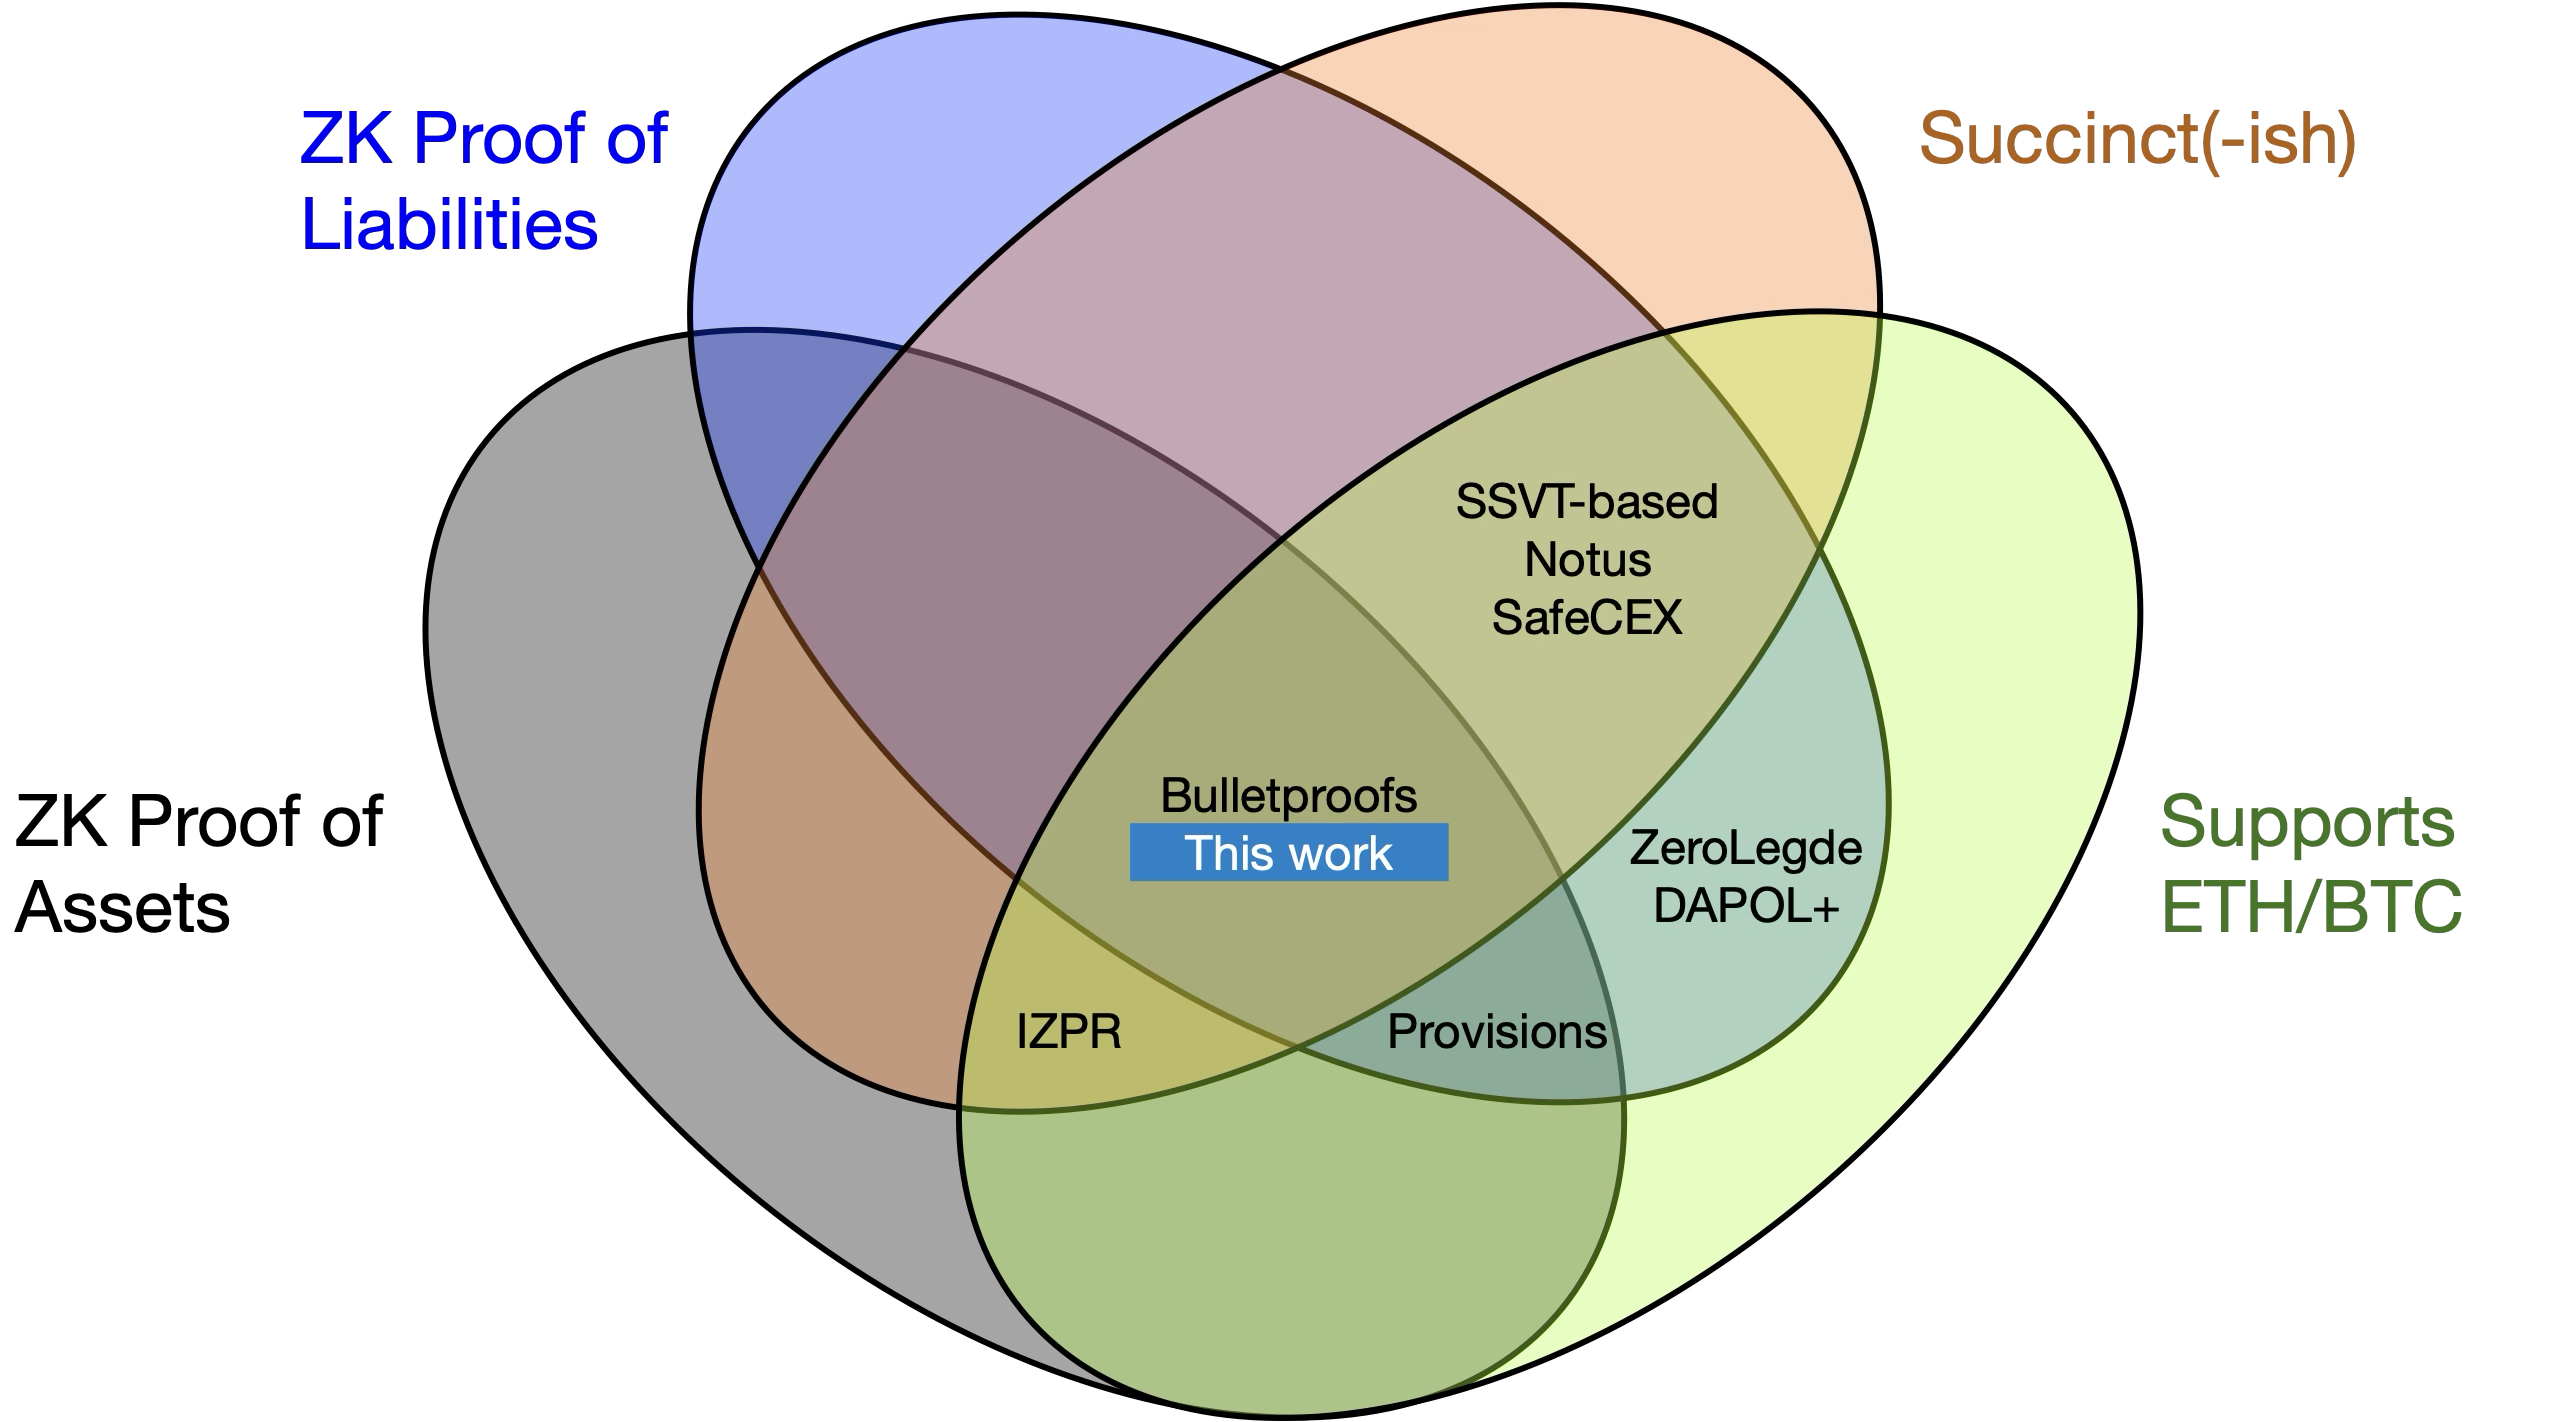
\includegraphics[scale=0.09]{venn.png}
    \end{columns}
  \end{frame}

  \subsection{Proof of Liabilities}
  \begin{frame}{Proof of Liabilities}
    Recall the problem
    \begin{itemize}
      \item Each user's balance is included in the proof
      \item The summation of all balances (total liability) is correct
      \item Each balance is in a specified range (range proof)
    \end{itemize}
    \visible<2->{Intuition
      \begin{columns}
      \column{0.4\textwidth}
        \begin{itemize}
        \item Interpolate a polynomial with balances
        \item<3-> Construct an accumulative polynomial
        \item<4-> Open the evaluation point for each user
        \end{itemize}
      \column{0.6\textwidth}
        $$
        \begin{matrix}
            \visible<3->{f_\mathsf{liab}(X): & r_1 & r_2 & \dots & r_{n-1} & r_n} \\
            p(X): & \mathsf{bal}_1 & \mathsf{bal}_2 & \dots & \mathsf{bal}_{n-1} & \mathsf{bal}_n \\
        \end{matrix}
        $$
      \end{columns}
    }
  \end{frame}

  \begin{frame}{Proof of Liabilities Example}
    \begin{table}
    \begin{tabular}{|m{2cm}|m{1cm}|m{1cm}|m{1cm}|m{1cm}|}
    \hline
    User & Alice & Bob & Charlie & David \\
    \hline
    Balance & 10 & 12 & 9 & 7 \\
    \hline
    \end{tabular}
    \caption{User Balances}
    \end{table}
    
    \visible<2->{
      \begin{table}
      \begin{tabular}{|m{2cm}|m{1cm}|m{1cm}|m{1cm}|m{1cm}|}
        \hline
        \diagbox[width=2.4cm]{Poly}{$X$} & 0 & 1 & 2 & 3 \\
        \hline
        $f_\mathsf{liab}(X)$ & 38 & 28 & 16 & 7 \\
        \hline
        $p(X)$ & 10 & 12 & 9 & 7 \\
        \hline
      \end{tabular}
      \caption{Polynomials}
      \end{table}
    }
    
    \visible<3->{
      \centering
      \begin{itemize}
          \item $f(X)=p(X),X=n-1$ \visible<4->{$\Rightarrow \frac{f(X)-p(X)}{X-(n-1)}=q_1(X)$}
          \item $f(X)=p(X)+f(X+1),\forall X\in[0,n-1)$ \visible<4->{$\Rightarrow \frac{f(X)-p(X)-f(X+1)}{X(X-1)(X-2)\cdots[X-(n-2)]}=q_2(X)$}
      \end{itemize}
    }
  \end{frame}

  \begin{frame}{Range Proof}
    \begin{itemize}
    \item Prove a value $x\in[0,2^k)$
    \item Prevent attacks by overflowing the liabilities and inserting negative values
    \item Binary decomposition\footnotemark
    \begin{itemize}
        \item $\overline{z}=\{z_1,z_2,\dots,z_k\},x=2^0\cdot{z_1}+2^1\cdot{z_2}+\dots+2^{k-1}\cdot{z_k}$
        \item $x=z_1+2\cdot(z_2+2\cdot(z_3+2\cdot(z_4+\dots)))$
    \end{itemize}
    \begin{table}
    \resizebox{0.9\textwidth}{!}{
        \begin{tabular}{|c|c|c|c|c|c|c|c|}
        \hline
        & $2^0$ & $2^1$ & $2^2$ & $2^3$ & $\dots$ & $2^{k-2}$ & $2^{k-1}$ \\
        \hline
        $\overline{z}$ & $z_1$ & $z_2$ & $z_3$ & $z_4$ & \dots & $z_{k-1}$ & $z_k$ \\
        \hline
        $\lambda$ & $z_1+2(z_2+\dots)$ & $z_2+2(z_3+\dots)$ & $z_3+2(z_4+\dots)$ & $z_4+2(z_5+\dots)$ & $\dots$ & $z_{k-1}+2z_k$ & $z_k$ \\
        \hline
        \end{tabular}
    }
    \end{table}
    \end{itemize}
    \vspace{-6.5em}
    \visible<2->{
      \begin{example}
        \vspace{-1em}
        \begin{table}
          \begin{tabular}{|c|c|c|c|c|}
          \hline
          & $2^0$ & $2^1$ & $2^2$ & $2^3$ \\
          \hline
          $x=13$ & $\lambda_0=1$ & $\lambda_1=0$ & $\lambda_2=1$ & $\lambda_3=1$ \\
          \hline
          $f_\mathsf{range}(X)$ & 13 & 6 & 3 & 1 \\
          \hline
          & $f_\mathsf{range}(0)$ & $f_\mathsf{range}(1)$ & $f_\mathsf{range}(2)$ & $f_\mathsf{range}(3)$ \\
          \hline
          \end{tabular}
        \end{table}
        \vspace{-1em}
        \begin{itemize}
          \item[]\begin{itemize}
          \item $f_\mathsf{range}(X)\in\{0,1\},X=k-1$
          \item $f_\mathsf{range}(X)-2\cdot f_\mathsf{range}(X+1)\in\{0,1\},X\in[0,k)$
        \end{itemize}
        \end{itemize}
      \end{example}
    }
    
    \footnotetext[1]{\url{https://hackmd.io/@dabo/B1U4kx8XI}}
  \end{frame}

  \begin{frame}{Proof of Liability + Range Proof}
    \begin{table}
    \begin{tabular}{|m{2cm}|m{1cm}|m{1cm}|m{1cm}|m{1cm}|}
    \hline
    \diagbox[width=2.4cm]{Poly}{$X$} & 0 & 1 & 2 & 3 \\
    \hline
    $f_\mathsf{liab}(X)$ & 38 & 28 & 16 & 7 \\
    \hline
    $p(X)$ & 10 & 12 & 9 & 7 \\
     & 5 & 6 & 4 & 3 \\
     & 2 & 3 & 2 & 1 \\
     & 1 & 1 & 1 & 0 \\
    \hline
    \end{tabular}
    \end{table}
    \visible<2->{
    The degree of $p(X)$ is proportional to the size of the range proof
    \begin{itemize}
      \item The largest set of the roots we can use is $2^{32}$
      \item One million $\approx$ $2^{20}$
      \item \alert{We can only prove values in $[0,2^{12})$}
    \end{itemize}
    }
    \visible<3->{
    Solution
    \begin{itemize}
      \item Break the range polynomial
    \end{itemize}
    }
  \end{frame}

  \begin{frame}{Proof of Liability + Range Proof}
    \begin{table}
      \begin{tabular}{|m{2cm}|m{1cm}|m{1cm}|m{1cm}|m{1cm}|}
      \hline
      \diagbox[width=2.4cm]{Poly}{$X$} & 0 & 1 & 2 & 3 \\
      \hline
      $f_\mathsf{liab}(X)$ & 38 & 28 & 16 & 7 \\
      \hline
      $p_1(X)$ & 10 & 12 & 9 & 7 \\
      \hline
      $p_2(X)$ & 5 & 6 & 4 & 3 \\
      \hline
      $p_3(X)$ & 2 & 3 & 2 & 1 \\
      \hline
      $p_4(X)$ & 1 & 1 & 1 & 0 \\
      \hline
      \end{tabular}
    \end{table}
    \begin{itemize}
      \item $f_\mathsf{liab}(n-1)=p_1(n-1)$
      \item $f_\mathsf{liab}(X)=f_\mathsf{liab}(X+1)+p_1(X),X\in[0,n-1)$
      \item $p_k(X)\in\{0,1\}$
      \item $p_i(X)-2p_{i+1}(X)\in\{0,1\}$
    \end{itemize}
    \visible<2->{\alert{Clash attack: count the same amount only once}}
  \end{frame}

  \begin{frame}{Clash Attack}
    \begin{table}
      \begin{tabular}{|m{2cm}|m{1cm}|m{1cm}|m{1cm}|m{1cm}|}
      \hline
      \diagbox[width=2.4cm]{Poly}{$X$} & 0 & 1 & 2 & 3 \\
      \hline
      $f_\mathsf{liab}(X)$ & 38 & 28 & 16 & 7 \\
      \hline
      $p_1(X)$ & 10 & 12 & 9 & 7 \\
      \hline
      $p_2(X)$ & 5 & 6 & 4 & 3 \\
      \hline
      $p_3(X)$ & 2 & 3 & 2 & 1 \\
      \hline
      $p_4(X)$ & 1 & 1 & 1 & 0 \\
      \hline
      \textcolor{blue}{$u(X)$} & A & B & C & D \\
      \hline
      \end{tabular}
    \end{table}
    \begin{itemize}
      \item $p_k(X)\in\{0,1\}$
      \item $p_i(X)-2p_{i+1}(X)\in\{0,1\}$
      \item $f_\mathsf{liab}(n-1)=p_1(n-1)$
      \item $f_\mathsf{liab}(X)=f_\mathsf{liab}(X+1)+p_1(X),X\in[0,n-1)$
      \item \textcolor{blue}{For each user $t$, $p_1(t)=\mathsf{bal}_t$, $u(t)=\mathsf{uid_t}$}
    \end{itemize}      
  \end{frame}

  \subsection{Proof of Assets}

  \begin{frame}{Proof of Assets}
    Recall the problem
    \begin{itemize}
      \item The exchange proves the ownership of some wallet accounts
      \item The total asset is the sum of these accounts
    \end{itemize}
    \visible<2->{
      \begin{block}{Preliminaries}
        \begin{itemize}
          \item Wallet address = $\mathsf{Hash}(\mathsf{pk})$
          \item $\mathsf{pk}=g^\mathsf{sk}$, where $g$ is a generator of an elliptic curve group (for Bitcoin and Ethereum, the curve is \secp; for the PCS, the curve is \bls)
          \item Secured by the discrete logarithm assumption
        \end{itemize}
      \end{block}
    }
  \end{frame}

  \begin{frame}{Proof of Assets}
    Intuition
    \begin{itemize}
      \item Publish some public keys as an anonymity set $\{\mathsf{pk}_i\}$
      \item<2-> Construct a selector polynomial $s(X)$ where each evaluation is in $\{0,1\}$
      \item<3-> Construct an accumulative polynomial
    \end{itemize}
    \resizebox{0.98\textwidth}{!}{
      $
      \begin{matrix}
          & \mathsf{pk}_1 & \mathsf{pk}_2 & \mathsf{pk}_3 & \dots & \mathsf{pk}_{n-1} & \mathsf{pk}_n \\
          b(X): & \mathsf{bal}_1 & \mathsf{bal}_2 & \mathsf{bal}_3 & \dots & \mathsf{bal}_{n-1} & \mathsf{bal}_n \\
          \visible<2->{s(X): & s_1 & s_2 & s_3 & \dots & s_{n-1} & s_n} \\
          \visible<3->{f_\mathsf{assets}(X): & r_1 & r_2 & r_3 & \dots & r_{n-1} & r_n} \\
          \visible<3->{ & s_1\cdot\mathsf{bal}_1+r_2 & s_2\cdot\mathsf{bal}_2+r_3 & s_3\cdot\mathsf{bal}_3+r_4 & \dots & s_{n-1}\cdot\mathsf{bal}_{n-1}+r_n & s_n\cdot\mathsf{bal}_n} \\
      \end{matrix}
      $
    }
    \visible<4->{\alert{How to construct such a selector polynomial in ZK?}}
  \end{frame}

  \begin{frame}{Disjunctive $\Sigma$-Protocol (OR Proof)}
    \begin{block}{OR Proof}
      Prove the claiming statement is $R_1$ or $R_2$ without telling which case it is.
    \end{block}
    \procedureblock{}{
      \mathcal{P} \< \< \mathcal{V}
      \\[0.1\baselineskip][\hline] \\[-0.5\baselineskip]  
      c_2\stackrel{\$}{\leftarrow}\{0,1\}^t \\
      [-0.5\baselineskip]
      \< \sendmessageright*{m_1,m_2} \\
      [-0.5\baselineskip]
      \<\< c\stackrel{\$}{\leftarrow}\{0,1\}^t \\
      [-0.5\baselineskip]  
      \< \sendmessageleft*{c} \\
      [-0.5\baselineskip]
      c_1=c\oplus c_2 \\
      [-0.5\baselineskip]
      \< \sendmessageright*{r_1,r_2,c_1,c_2} \\
      [-0.5\baselineskip]
      \<\< \text{check } \\
      [-0.3\baselineskip]
      \<\< \text{(i) }c\stackrel{?}{=}c_1\oplus c_2 \\
      [-0.3\baselineskip]
      \<\< \text{(ii) }(m_1,c_1,r_1)\in R_1 \\
      [-0.3\baselineskip]
      \<\< \text{(iii) }(m_2,c_2,r_2)\in R_2
    }
  \end{frame}

  \begin{frame}{Proof of Assets + OR Proof}
    \alert{A useful observation:} the previous proof of assets has composite statements:
    \begin{enumerate}
      \item The selector $s_i$ is 1 and prove the knowledge of the corresponding private key
      \begin{itemize}
        \item $\gb^{s_i}=\gb^1$ (in \bls)
        \item the knowledge of $\mathsf{sk}_i$ (in \secp)
      \end{itemize}
      \item The selector $s_i$ is 0
      \begin{itemize}
        \item $\gb^{s_i}=\gb^0$ (in \bls)
      \end{itemize}
    \end{enumerate}
    \visible<2->{
      \alert{Can we open the commitment to the evaluation without revealing the evaluation itself?}
    }
    \vspace{-3em}
    \visible<3->{
      \begin{block}{PCS Extension} 
        Open the committed evaluation $\gb^{x}$~\footnote{See Section B of the paper.}.
      \end{block}
    }
  \end{frame}

  \begin{frame}{Proof of Assets + OR Proof}
    \procedureblock[colspace=-5em]{}{
      \mathcal{P} \< \< \hspace{6em} \mathcal{V} \\
      \\[-0.5\baselineskip][\hline] \\[-0.5\baselineskip]  
      \dbox{
        \begin{subprocedure}\procedure{$s_i=1$}{
          c_2\stackrel{\$}{\leftarrow}\{0,1\}^l \< \< \\
          m_1^{(i)},m_1^{(ii)},m_2,r_2 \< \< \\
          \< \sendmessageright*[1.5cm]{m_1^{(i)},m_1^{(ii)},m_2} \< \\
          \< \< \sendmessageleft*[1.5cm]{c\stackrel{\$}{\leftarrow}\{0,1\}^l} \hspace{-2.5em} \\
          c_1=c\oplus c_2 \< \< \\
          \< \sendmessageright*[1.5cm]{r_1^{(i)},r_1^{(ii)},r_2,c_1,c_2} \< \\
          [-1\baselineskip]
        }
        \end{subprocedure}
      }
        \< \<
      \hspace{6em}
      \dbox{
        \begin{subprocedure}\procedure{$s_i=0$}{
          c_1\stackrel{\$}{\leftarrow}\{0,1\}^l \< \< \\
          m_1^{(i)},m_1^{(ii)},m_2,r_1^{(i)},r_1^{(ii)} \< \< \\
          \< \sendmessageright*[1.5cm]{m_1^{(i)},m_1^{(ii)},m_2} \< \\
          \< \< \sendmessageleft*[1.5cm]{c\stackrel{\$}{\leftarrow}\{0,1\}^l} \hspace{-2.5em} \\
          c_2=c\oplus c_1 \< \< \\
          \< \sendmessageright*[1.5cm]{r_1^{(i)},r_1^{(ii)},r_2,c_1,c_2} \< \\
          [-1\baselineskip]
        }
        \end{subprocedure}
      } \\
      [-0.1\baselineskip]
      \< \< \hspace{6em} \text{check }(m_1^{(i)},r_1^{(i)},c_1),(m_1^{(ii)},r_1^{(ii)},c_1), \\
      \< \< \hspace{6em} \text{      }(m_2,r_2,c_2) \\
    }
  \end{frame}

  \begin{frame}{Full Protocol of Proof of Assets}
    \begin{enumerate}
        \item Bootstrapping (pre-computing)
        \begin{enumerate}
            \item Interpolate selector polynomial $s(X)$
            \item Open the evaluations of $s(X)$
            \item Prove each evaluation is valid (the OR proof)
        \end{enumerate}
        \item Interpolate the balance polynomial $b(X)$
        \item Construct the accumulative polynomial $f_\mathsf{assets}(X)$
        \item Prove the polynomial constraints (accumulate assets) are correct
    \end{enumerate}
  \end{frame}

  \subsection{Proof of Solvency}

  \begin{frame}{Proof of Solvency}
    \begin{itemize}
      \item Run the Proof of Liabilities to output $f_\mathsf{liab}(X)$
      \item Run the Proof of Assets to output $f_\mathsf{assets}(X)$
      \item Open the evaluations of $f_\mathsf{liab}(0)$ and $f_\mathsf{assets}(0)$ and compute $\Delta=f_\mathsf{assets}(0)-f_\mathsf{liab}(0)$
      \item Prove $\Delta\ge{0}$ using the range proof
    \end{itemize}
  \end{frame}

  \subsection{Performance Evaluation}

  \begin{frame}{Benchmark Performance}
    Proof of assets
    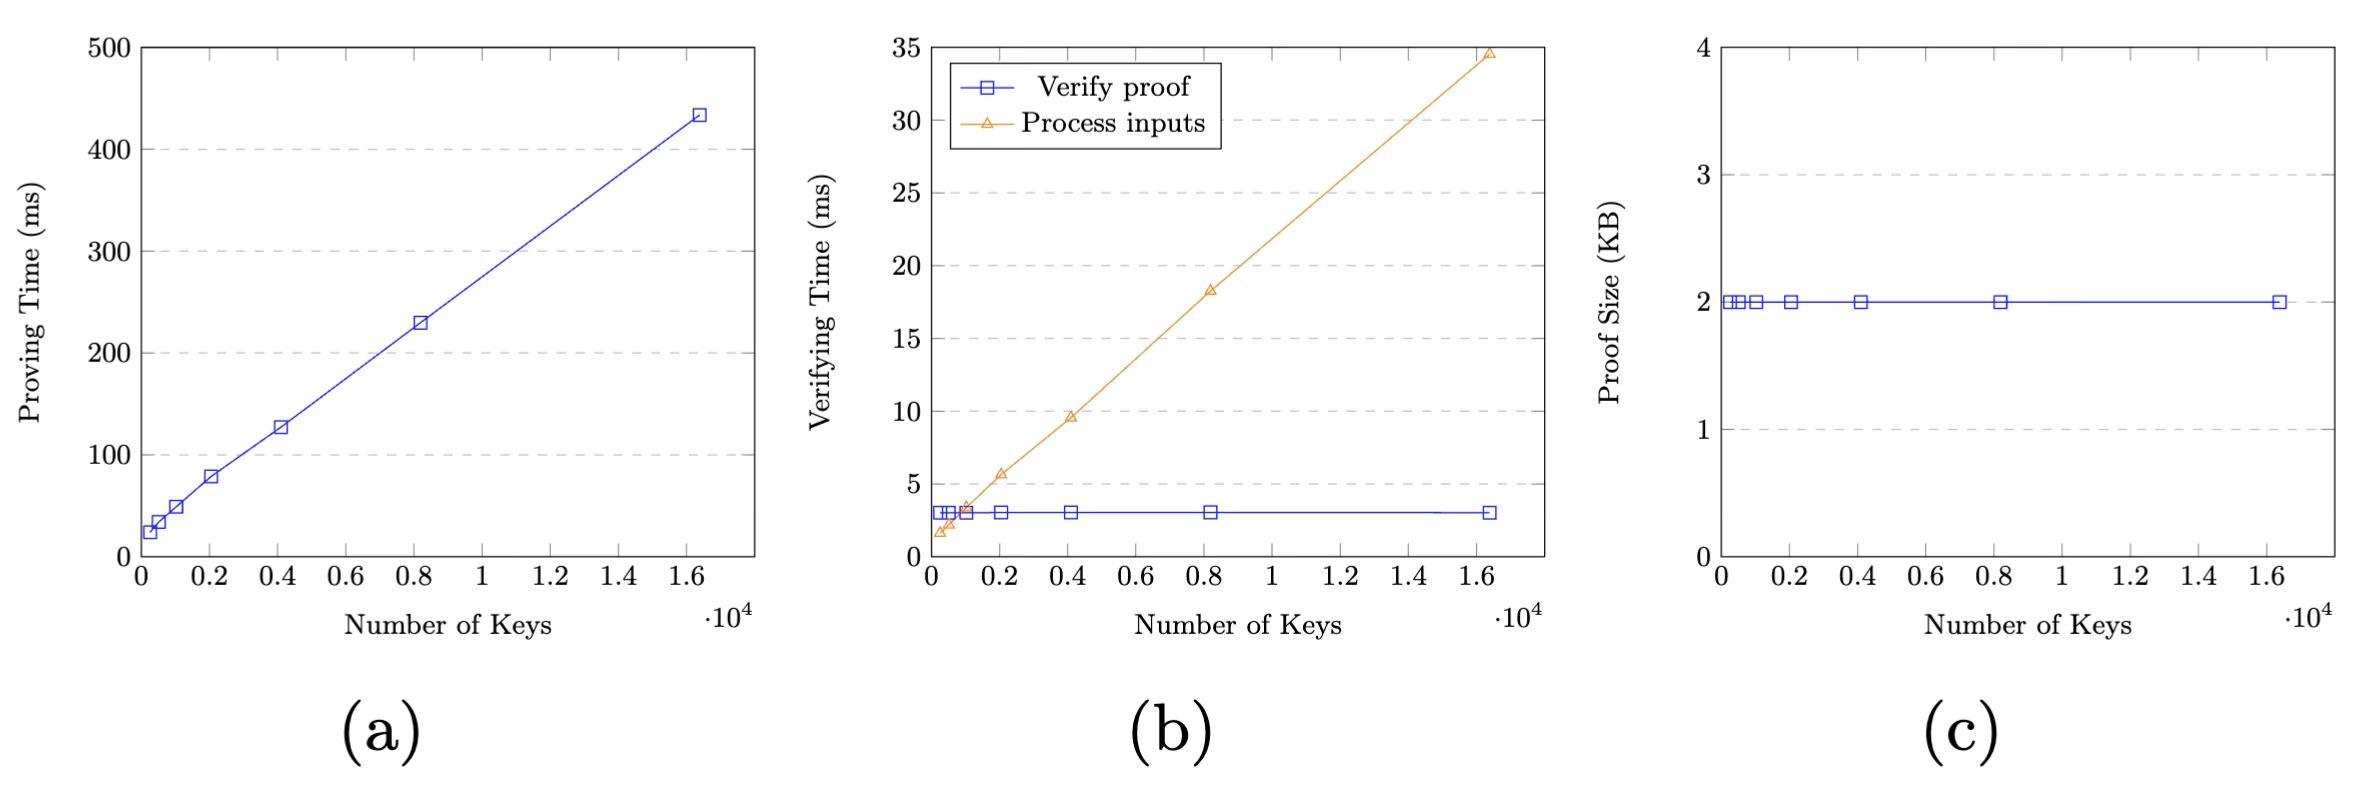
\includegraphics[scale=0.13]{poa.png}\\
    Proof of liability
    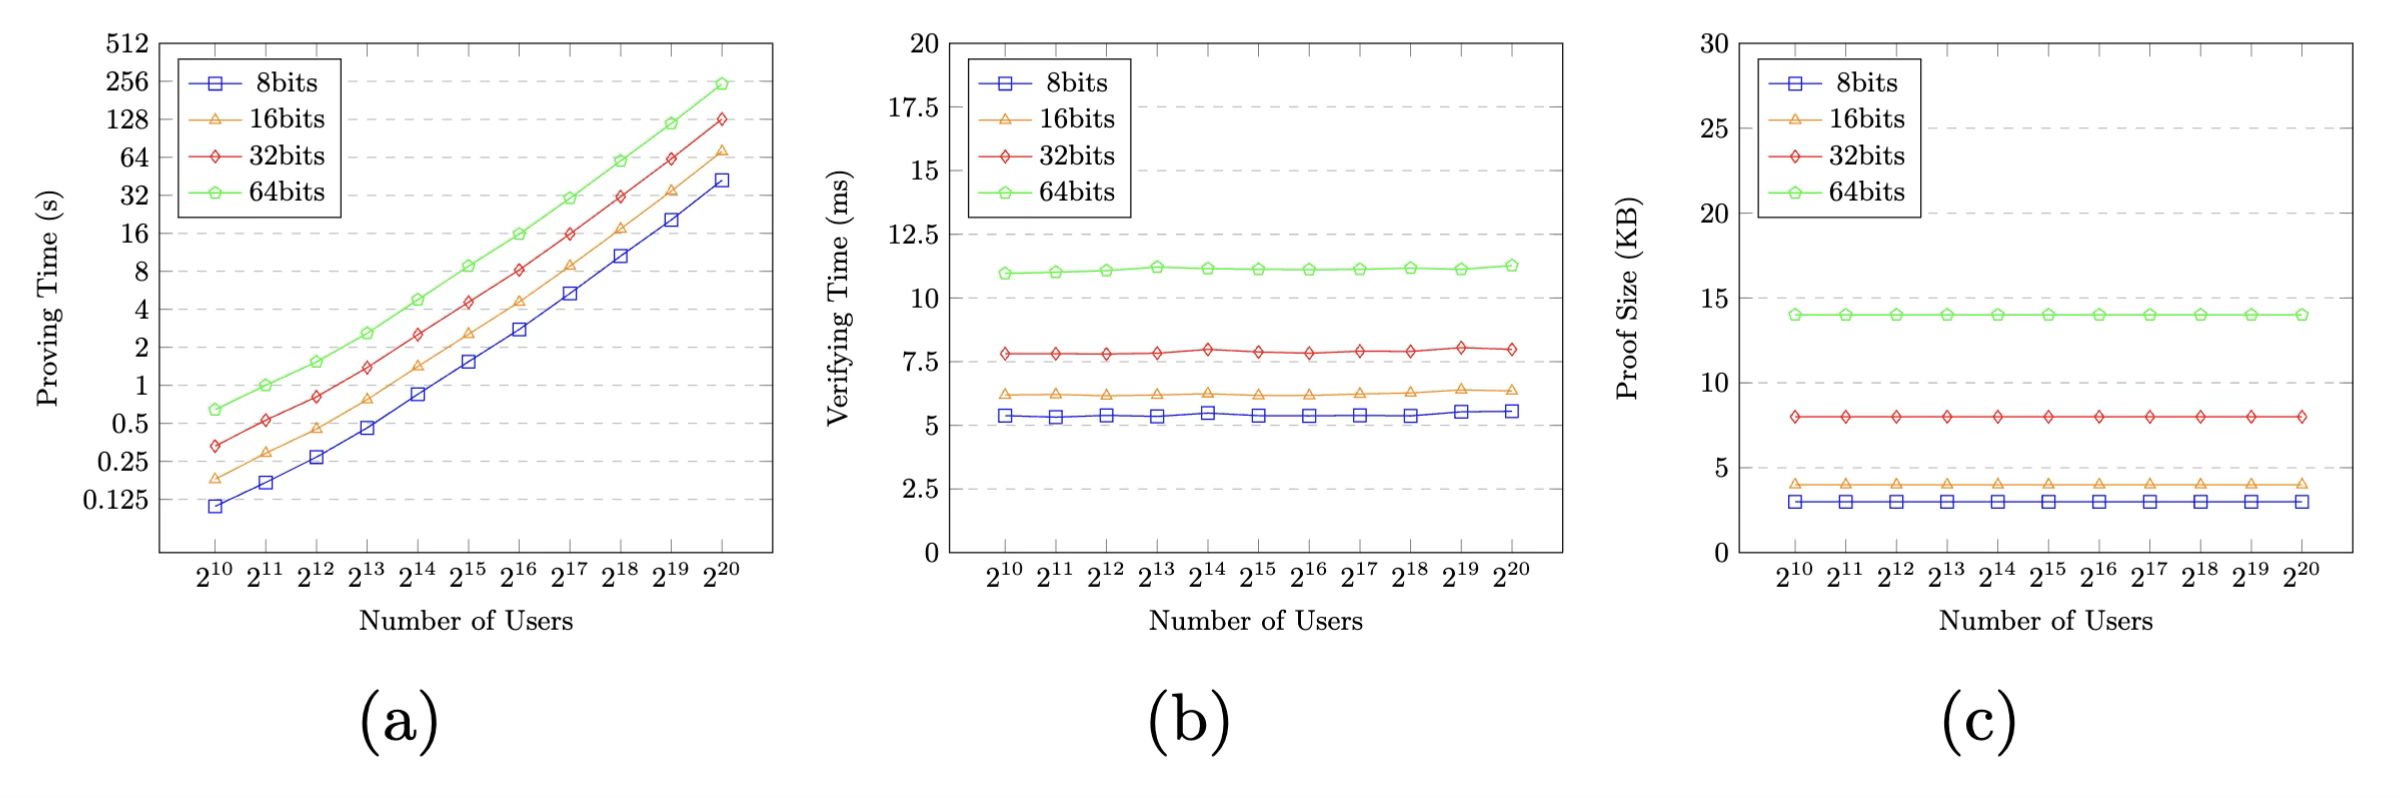
\includegraphics[scale=0.13]{pol.png}
  \end{frame}

% ==================================================

  \section{Outro}

  \subsection{Conclusion}

  \begin{frame}{Conclusion}
    \begin{itemize}
      \item This work is an almost succinct proof of solvency
      \item It is practical to be deployed for the real-world exchanges, implemented in Rust (\href{https://github.com/Shvier/proof-of-solvency}{https://github.com/Shvier/proof-of-solvency})
      \item Future work
      \begin{itemize}
          \item Multivariate polynomial for better performance
          \item Incremental update (folding schemes)
          \item Shorter range proof (lookup arguments) 
      \end{itemize}
    \end{itemize}
  \end{frame}

  \subsection{State of the Art in ZKP}

  \begin{frame}{State of the Art in ZKP}
    \begin{itemize}
      \item Applications
      \begin{itemize}
        \item In blockchain: zkRollup, zkBridge, zkEVM
        \item In other fields: zkML, zk program analysis, fight disinformation~\footnote{\url{https://rdi.berkeley.edu/zk-learning/assets/Lecture2-2023.pdf}}
      \end{itemize}
      \item Limitations
        \begin{itemize}
          \item Cost
          \item Performance
          \item Complication
        \end{itemize}
      \item Further reading
        \begin{itemize}
          \item \href{https://rdi.berkeley.edu/zk-learning/}{ZK MOOC}
          \item \href{https://vitalik.eth.limo/general/2019/09/22/plonk.html}{Vitalik's Blog}
          \item \href{https://toc.cryptobook.us/}{A Graduate Course in Applied Cryptography}
        \end{itemize}
    \end{itemize}
  
  \end{frame}

\end{document} 